% XeLaTeX can use any Mac OS X font. See the setromanfont command below.
% Input to XeLaTeX is full Unicode, so Unicode characters can be typed directly into the source.

% The next lines tell TeXShop to typeset with xelatex, and to open and save the source with Unicode encoding.

%!TEX TS-program = xelatex
%!TEX encoding = UTF-8 Unicode

\documentclass[12pt]{article}
\usepackage{geometry}                % See geometry.pdf to learn the layout options. There are lots.
\geometry{letterpaper}                   % ... or a4paper or a5paper or ... 

\geometry{left=1in}
\geometry{right=1in}
\geometry{bottom=1.9in}
\geometry{top=1in}

%
%Setting the font
%
\usepackage{times}

%
%Rotating tables (e.g. sideways when too long)
%
\usepackage{rotating}

%
%For multiple rows in tables
%
\usepackage{multirow}

% 
%Line numbering in verse environment
%
\usepackage{lineno} 

%
%Fancy-header package to modify header/page numbering (insert last name)
%
\usepackage{fancyhdr}
\pagestyle{fancy}
\lhead{} 
\chead{} 
\rhead{Quan \thepage} 
\lfoot{} 
\cfoot{} 
\rfoot{} 
\renewcommand{\headrulewidth}{0pt} 
\renewcommand{\footrulewidth}{0pt} 
%To make sure we actually have header 0.5in away from top edge
%12pt is one-sixth of an inch. Subtract this from 0.5in to get headsep value
\setlength{\headsep}{1in}

\usepackage{setspace}
\doublespacing

\usepackage{booktabs}
\usepackage[american]{babel}
\usepackage{csquotes}
\usepackage[style=mla]{biblatex}
\usepackage{url}
\usepackage[parfill]{parskip}
\usepackage{listings}
 \usepackage{float}

\usepackage{titlesec}
\usepackage{amsmath}

\usepackage{xcolor}

\lstset{language=python}
\lstset{breaklines}
\definecolor{mygreen}{rgb}{0,0.6,0}
\definecolor{mygray}{rgb}{0.5,0.5,0.5}
\definecolor{mymauve}{rgb}{0.58,0,0.82}

\lstset{numbers=left, 
numberstyle=\tiny, 
keywordstyle=\color{blue},
commentstyle=\color{mygreen},    % comment style
rulecolor=\color{black},
frame=shadowbox, 
rulesepcolor=\color{red!20!green!20!blue!20},
stringstyle=\color{mymauve},     % string literal style
title=\lstname,
showspaces=false,
showstringspaces=false
}


\title{}
\author{}
\date{}                                           % Activate to display a given date or no date

\addbibresource{bib.bib}
\begin{document}

\begin{flushleft}
%%%%First page name, class, etc
Shengjie Quan\\
Professor: Jihun Hamm\\
CSE 3521	 \\
\today \\
\end{flushleft}

%%%%Title
\begin{center}
Response to Homework 2
\end{center}

%%%%Changes paragraph indentation to 0.5in
\setlength{\parindent}{0.5in}

\begin{singlespace}

\begin{enumerate}

\item 
	Below is a belief-state space diagram to the erratic and sensorless vacuum with an unknown initial state problem. The problem will not for certain to achieve the goal because according to the diagram, whatever actions take, the problem will only looping amaong some belief states and will never get to a belief state that only contain goals. Thus, for this problam, the goal will not achieve for certain.
	\begin{figure}[h]
	\centering
	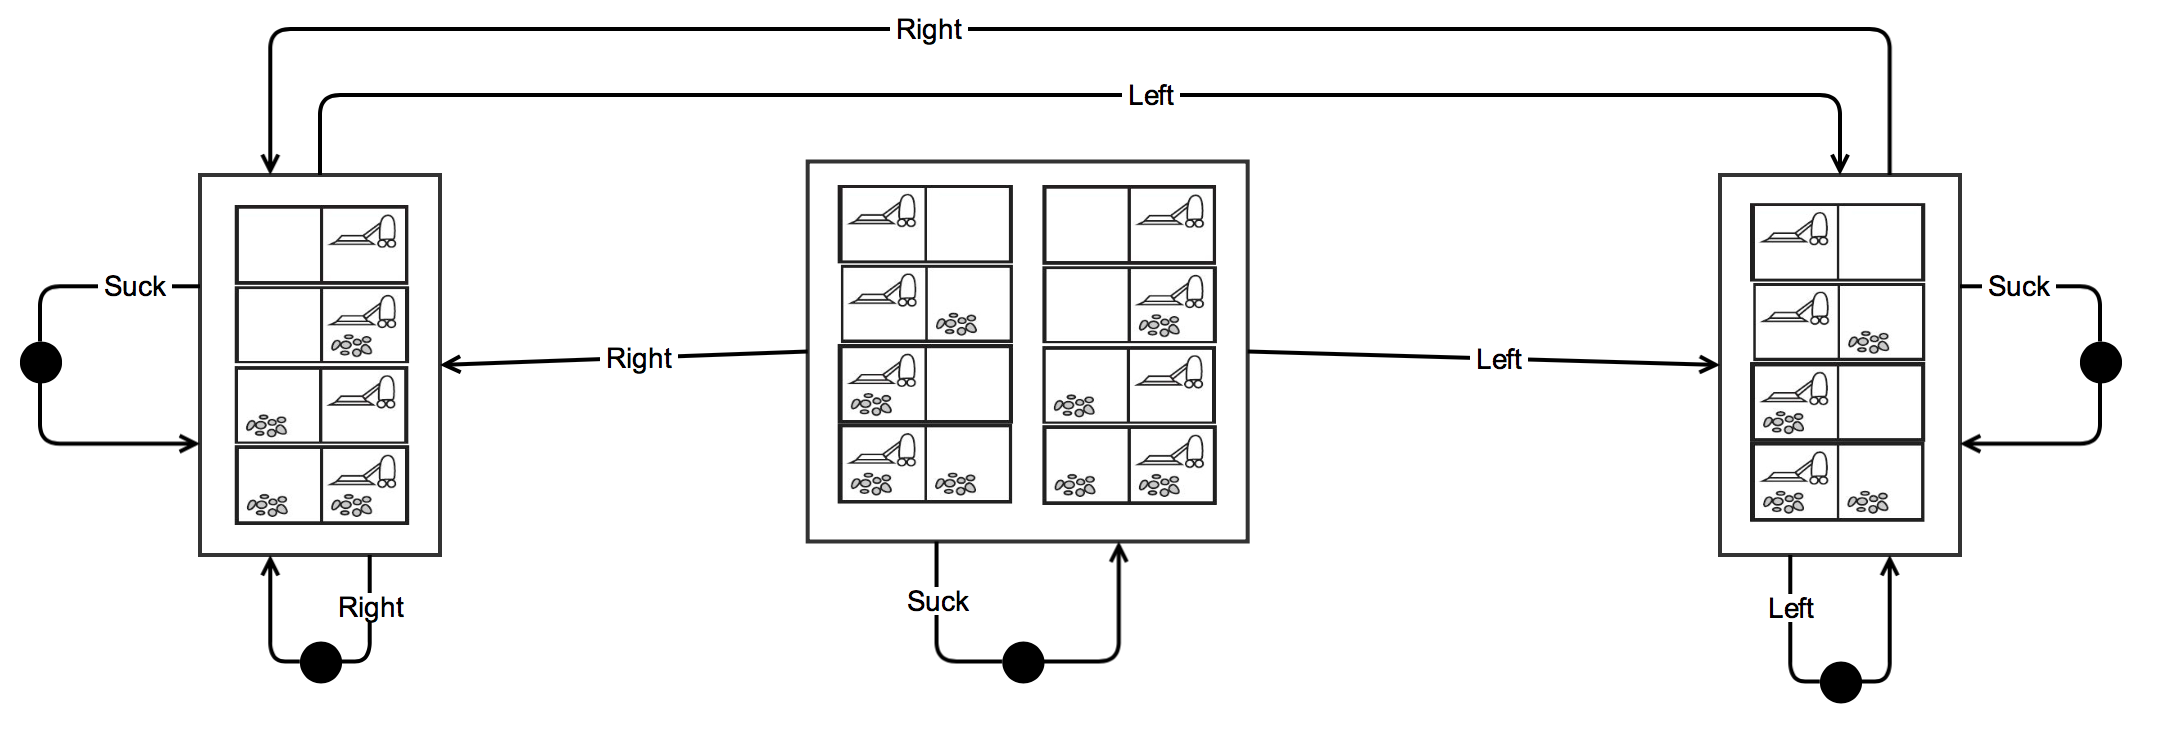
\includegraphics[width=1.1\textwidth]{b} 
	\end{figure}

\item
	\begin{itemize}
	\item[(a.)] For state 1, $h^* = 3$ since a sequence of solving is $S->R->S$.\\
	For state 2, $h^*(s) = 3$ since a sequence of solving is $S->L->S$.\\
	For state 3, $h^*(s) = 1$ since a sequence of solving is $S$.\\
	For state 4, $h^*(s) = 2$ since a sequence of solving is $L->S$.\\
	For state 5, $h^*(s) = 2$ since a sequence of solving is $R->S$.\\
	For state 6, $h^*(s) = 1$ since a sequence of solving is $S$.\\
	For state 7, $h^*(s) = 0$ since it is already at the goal state.\\
	For state 8, $h^*(s) = 0$ since it is already at the goal state.\\
	\item[(b.)] For the initial state, $h(b) = 3$ according to (a.).
	\item[(c.)] According to the graph on p.19 of lecture 7, if we treat a belif state as a node in the graph, then the actual shortest cost from the initial state node to any of the goal state node is 4 (A sequence of action could be $L->S->R->S$ or $R->S->L->S$). So for the initial state $h(b)$ under estimate the cost. And it is easy to see that this is true for all nodes. Thus, $h(b)$ is an admissible heuristid for this problem.
	\end{itemize}
\item
	\begin{itemize}
	\item[(a.)] The minimax value are labled on the tree below. The solution is the path circled out in the tree.
	\begin{figure}[h]
	\centering
	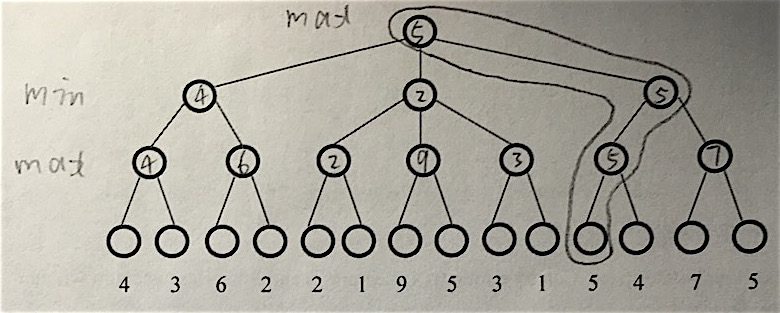
\includegraphics[width=0.9\textwidth]{3a} 
	\end{figure}
	\item[(b.)] The minimax value range are labled on the tree below. The nodes with cross are the roots of the branches being pruned.
	\begin{figure}[h]
	\centering
	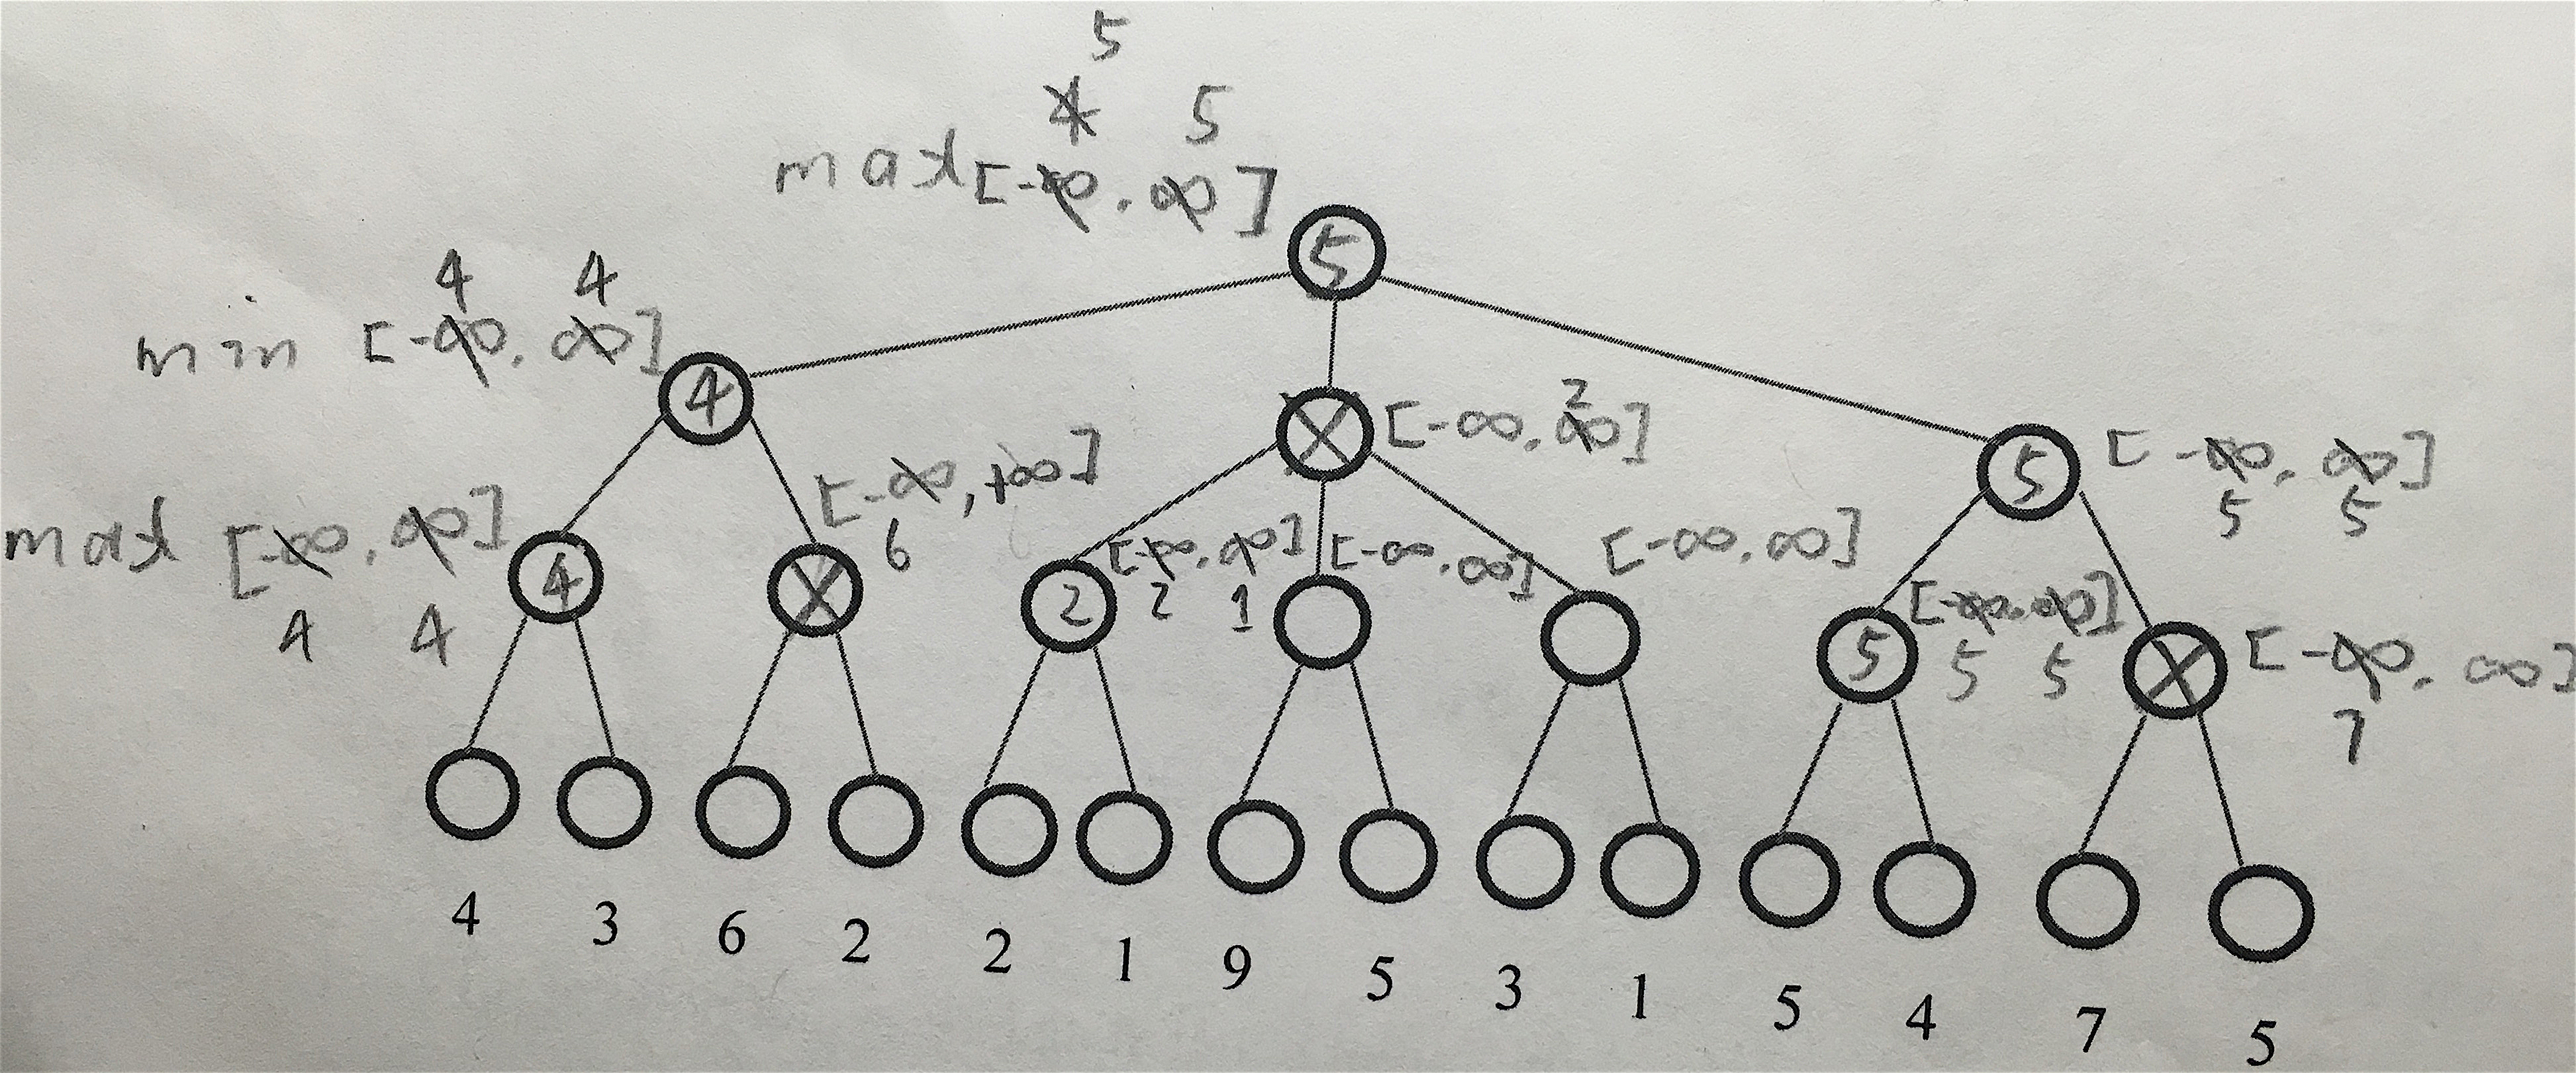
\includegraphics[width=0.9\textwidth]{3b} 
	\end{figure}
	\end{itemize}
\end{enumerate}
\end{singlespace}

\clearpage

\printbibliography
\end{document}  